\documentclass[twocolumn]{exam}
\usepackage[a4paper, margin=1cm, bottom=2cm]{geometry}
\usepackage{graphicx}
\usepackage{amsmath}
\usepackage{amssymb}
\usepackage{xcolor}
\usepackage{listings}
%\usepackage{fancyhdr}

\usepackage{tikz}
\usepackage{lastpage}
\usetikzlibrary{graphs, graphdrawing, bending}
\usegdlibrary{layered}

\definecolor{mGreen}{rgb}{0,0.6,0}
\definecolor{mGray}{rgb}{0.5,0.5,0.5}
\definecolor{mPurple}{rgb}{0.58,0,0.82}
\definecolor{backgroundColour}{rgb}{0.95,0.95,0.92}

\lstdefinestyle{CStyle}{
    breakatwhitespace=true,         
    breaklines=true,                 
    keepspaces=false,                                
    showspaces=false,                
    showstringspaces=false,
    showtabs=false,                  
    tabsize=2,
    language=C
}

\printanswers

% Define the \coursegroup command
\newcommand{\coursegroup}{A}
\newcommand{\examinfo}{BLM2011 Statistics and Probability Calculations, Make-up (Bütünleme) Exam, 2023 - 2024 Fall, 22 Dec 2023, Key \coursegroup}



\footer{}{}{\examinfo, Page \thepage/\pageref{LastPage}}
%\footer{}{}{\examinfo, Page \thepage}


\begin{document}


\examinfo


\noindent 
\fbox{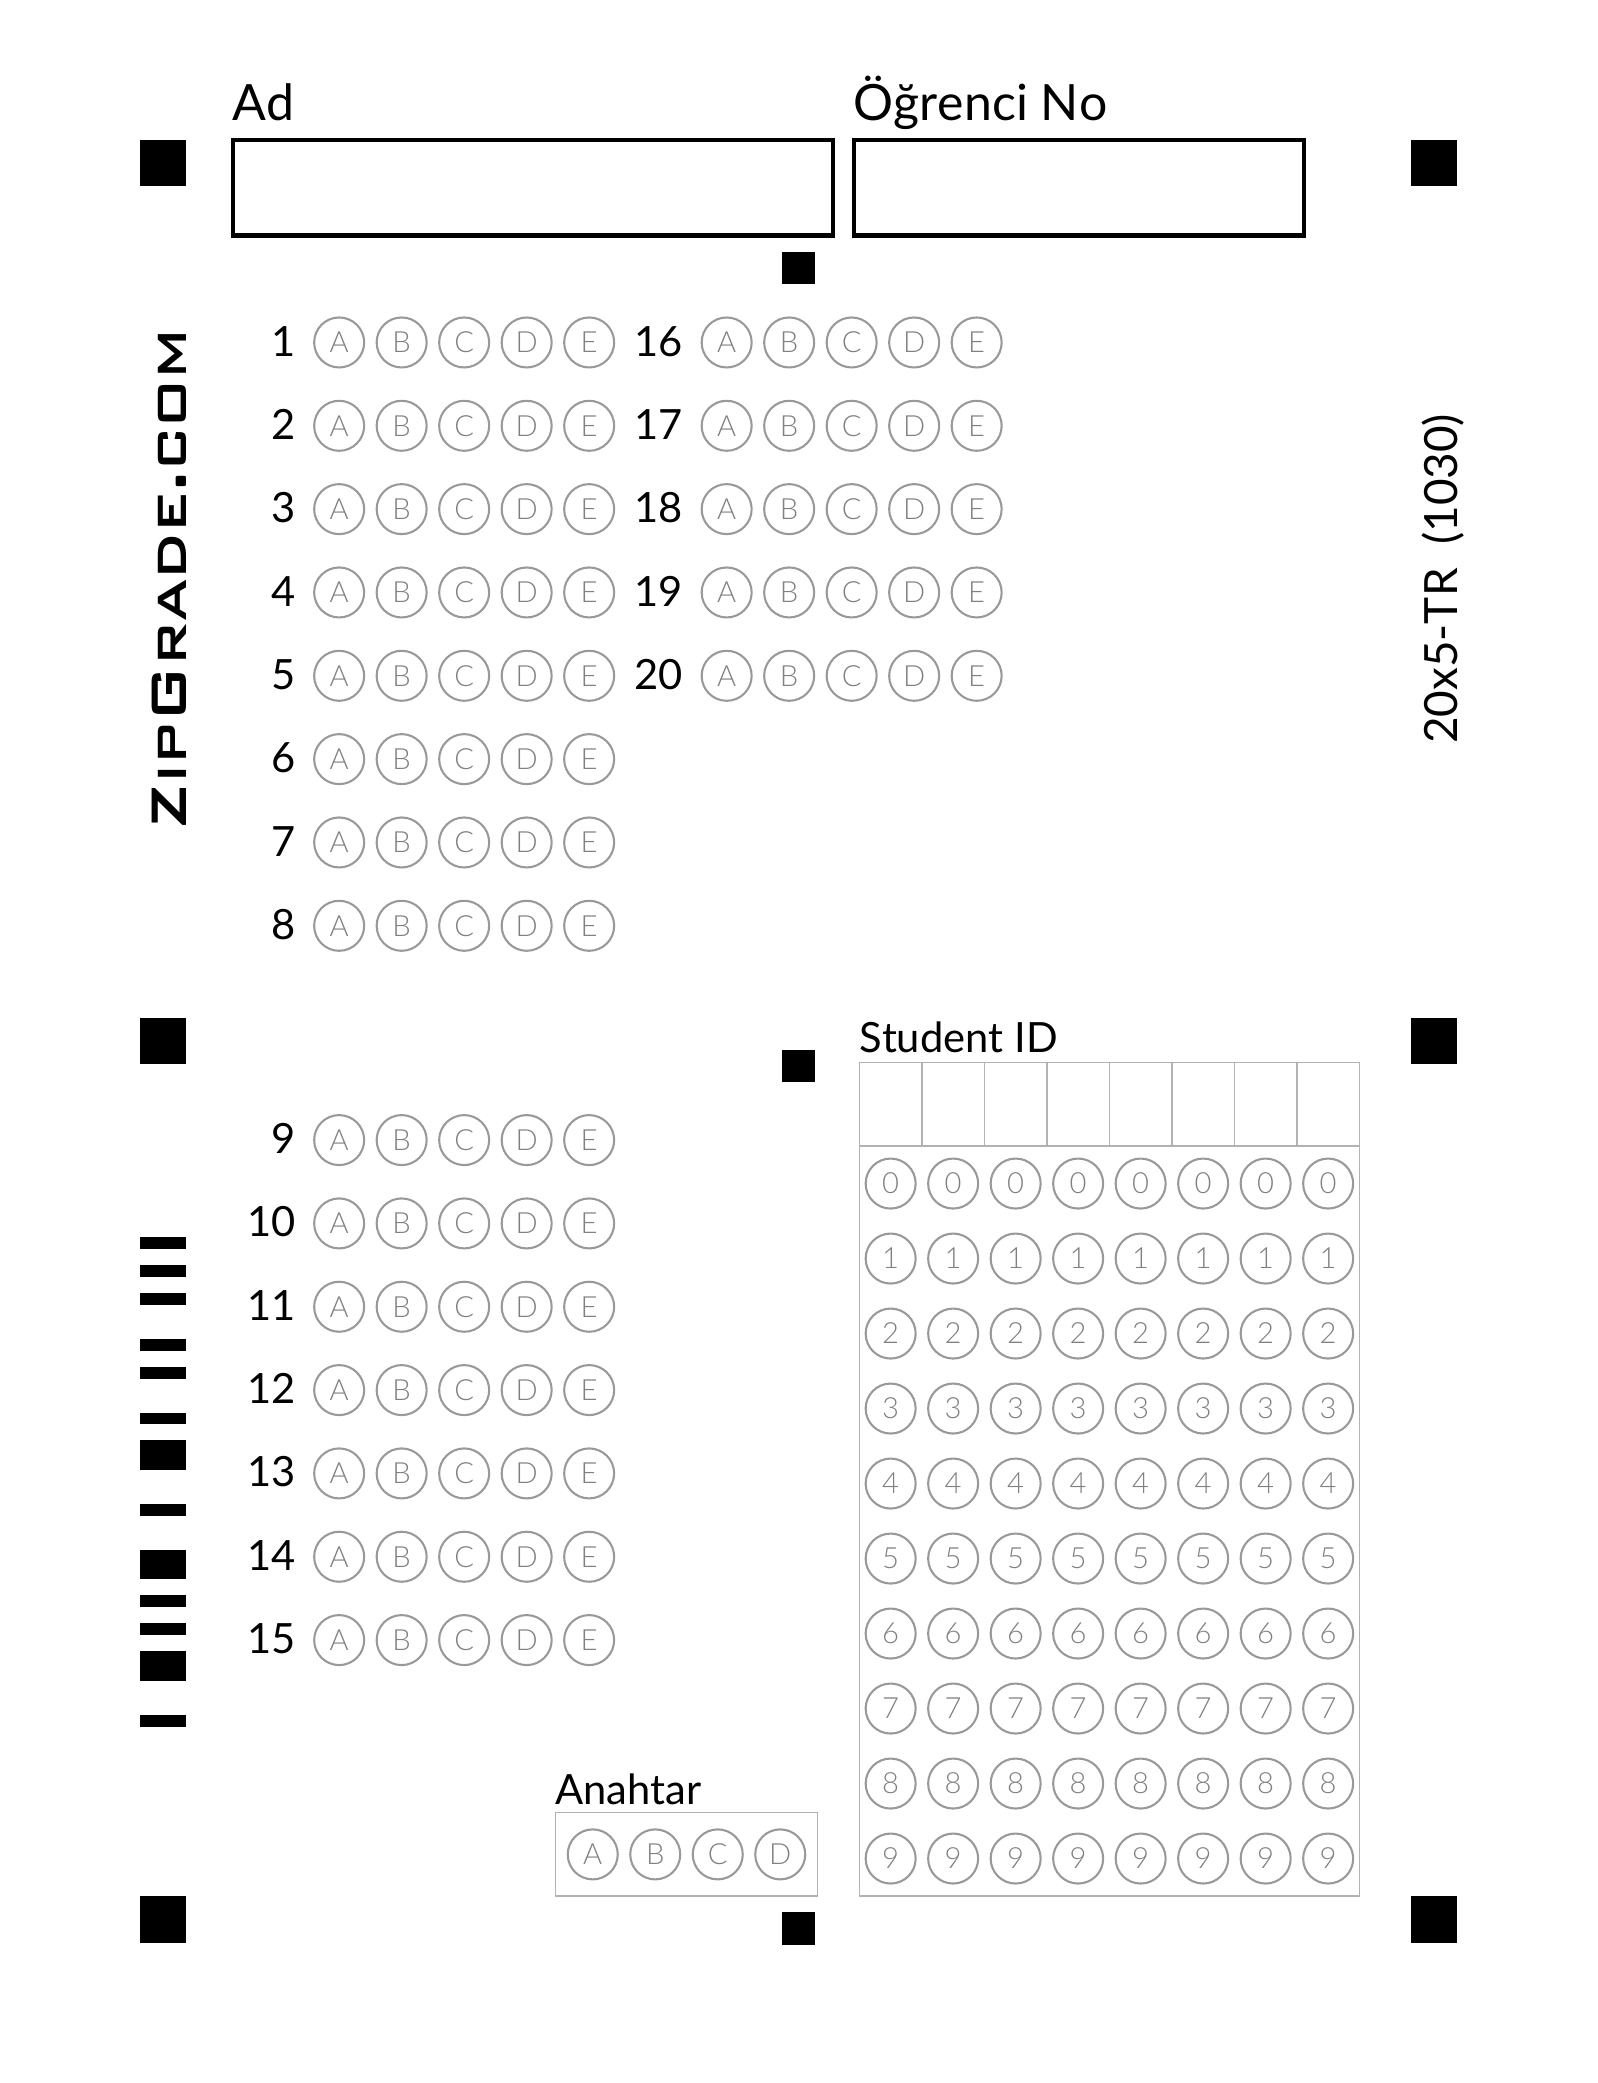
\includegraphics[width=0.9\linewidth]{1030.png}}
\newline
\textbf{Instructions}: 
\begin{itemize}
    \item Mark your answers on the answer key. Do not write/draw anything other than answer markings in the answer key area, as it can confuse the optical scanner.
    \item Scratch paper can be used. Submit your scratch paper at the end of the exam. Taking it outside is prohibited.
    \item You can make scratch notes on the question paper, but do not make any markings that indicate your answer. Such markings will be treated as an attempt to cheat (points for that question will be canceled). Similarly, do not write/make markings on the scratch paper that match a question with its answer. It will be treated in the same manner.
    \item Write and mark your name and number in the relevant fields on the answer key. Make sure you have correctly marked the 'Key' field on the answer key. The exam will be read optically.
    \item You may ask for the meanings of words you do not know in English/Turkish. You can ask questions you do not understand.
    \item There may be incorrect questions. Report any questions you suspect to the exam supervisor. They will be checked after the exam and canceled if there is an error. Sometimes the same answer is inadvertently printed for more than one option. In this case, mark the alphabetically first option and inform the exam supervisors. They will adjust the reader program accordingly.
    \item Calculators can be used.
    \item All questions are worth equal points.
    \item Standard Normal Distribution Cumulative Distribution Values: $\Phi(-1) \approx 0.16$, $\Phi(1) \approx 0.84$, $\Phi(2.24) \approx 0.98$, $\Phi(2.18) = 0.9854$, $\Phi(2.29) = 0.9890$
    \item Standard Normal Distribution Quantiles(Z-scores): $z_{0.10} = \Phi^{-1} (0.90) = 1.282$, $z_{0.05} = 1.645$,
    $z_{0.025} = 1.960$, $z_{0.01} = 2.326$, $z_{0.005} = 2.576$.
    \end{itemize}
    
     
% \begin{itemize}
%     \item Cevaplarınızı cevap anahtarına işaretleyiniz. Cevap anahtarı bölgesi içine cevap işaretlemeleri haricinde yazım/çizim yapmayınız, optik okuyucu programı şaşırtmaktadır.
%     \item Karalama kağıdı kullanılabilir. Karalama kağıdınızı sınav sonunda teslim ediniz. Dışarı çıkarmak yasaktır.
%     \item Soru kağıdına karalama yapabilirsiniz, ancak cevabınızı belli edecek herhangi bir işaretleme yapmayınız. Bu şekildeki işaretlemeler kopya verme girişimi muamelesi görecektir (sorudan alınan puan iptal edilecektir). Aynı şekilde karalama kağıdında bir soru ile cevabını eşleyen bir yazma/işaretleme yapmayınız. Aynı şekilde muamele görecektir.
%     \item İsminizi ve numaranızı cevap anahtarında ilgili alanlara yazınız ve işaretleyiniz. Cevap anahtarında 'Anahtar' alanınını doğru işaretlediğinizden emin olunuz. Sınav optik olarak okunacaktır.
%     \item İngilizce/Türkçe bilmediğiniz kelimeleri sorabilirsiniz. Anlamadığınız soruları sorabilirsiniz. 
%     \item Yanlış sorular olabilir. Sınav sorumlusuna şüphelendiğiniz soruları bildiriniz. Sınav sonrasında kontrol edilecek ve hata var ise iptal edilecektir. Yine bazen aynı cevap sehven birden fazla şıkka basılmaktadır. Bu durumda alfabetik olarak önce gelen şıkkı işaretleyiniz ve sınav görevlilerini durumdan haberdar ediniz. Sınav görevlileri okuyucu programı uygun ayarlayacaktır.
%     \item Hesap makinesi kullanılabilir.
%     \item Tüm sorular eşit puanlıdır.
% \end{itemize}


\textbf{Questions} (Each equal in points):

\begin{questions}
    




\question A company offers a referral bonus program. For each referred employee who stays at least 6 months, the referrer gets 500 dollars. If the probability that a referred employee stays for 6 months is 0.4, what is the expected bonus for referring one employee in dollars?

\begin{oneparchoices}
\correctchoice 200
\choice 500
\choice 100
\choice 0
\end{oneparchoices}

\begin{solution}
The expected bonus is \(E(X) = 0.4 \times 500 = 200\) dollars.
\end{solution}
    




\question A basketball player has a 70 percent chance of making each free throw. If she takes 10 free throws, what is the expected number of free throws she will make?

\begin{oneparchoices}
\correctchoice $7$ free throws
\choice $3$ free throws
\choice $10$ free throws
\choice $5$ free throws
\end{oneparchoices}

\begin{solution}
The expected number is \(E(X) = np = 10 \times 0.7 = 7\) free throws.
\end{solution}
    




\question A taxi company charges a flat rate of 3 dollars plus 2 dollars per mile. If the distance of a ride follows a uniform distribution between 1 and 5 miles, what is the expected cost of a ride in dollars?

\begin{oneparchoices}
\correctchoice 9
\choice 8
\choice 10
\choice 7
\end{oneparchoices}

\begin{solution}
The expected distance is the mean of the uniform distribution, \(\frac{1 + 5}{2} = 3\) miles. Thus, the expected cost is \(3 + 2 \times 3 = 9\) dollars.
\end{solution}
    



\end{questions}





\end{document}

